%%%%%%%%%%%%%%%%%%%%%%%%%%%%%%%%%%%%%%%%%%%%%%%%%%%%%%%%%%%%%%%%%%%%%%%%%%%%%%%
%%                                                                           %%
%%   Dr Derek Harter                                                         %%
%%   Profesor, Department of Computer Science                                %% 
%%   Texas A&M University - Commerce, USA                                    %%
%%                                                                           %%
%%%%%%%%%%%%%%%%%%%%%%%%%%%%%%%%%%%%%%%%%%%%%%%%%%%%%%%%%%%%%%%%%%%%%%%%%%%%%%%
%%%%     SETTING STARTS - DO NOT CHANGE Unless your TeX setting require so   %%
%%%%%%%%%%%%%%%%%%%%%%%%%%%%%%%%%%%%%%%%%%%%%%%%%%%%%%%%%%%%%%%%%%%%%%%%%%%%%%%
%%----------------------------------------------------------------------------------
% DO NOT Change this. It is the required setting letterpaper page, 11pt, onside print, book style
%%----------------------------------------------------------------------------------
\documentclass[letterpaper,11pt,oneside]{book}

%%-------------------------------------
%% Page margin settings - % half inch margin all sides (recommended)
%%-------------------------------------
\usepackage[margin=1.2in]{geometry} 

%%-------------------------------------
%% Font settings - % CM San or Ariel (recommended)
%%-------------------------------------
% Switch the following two line off: to revert back to default LaTex font (NOT recommended)
\usepackage{amsfonts}
\renewcommand*\familydefault{\sfdefault}

%%-------------------------------------
%% Math/Definition/Theorem/Algorithm packages settings 
%%-------------------------------------
\usepackage[cmex10]{amsmath}
\usepackage{amssymb}
\usepackage{amsthm}
\newtheorem{mydef}{Definition}
\newtheorem{mytherm}{Theorem}

%%-------------------------------------
%% Algorithms/Code Listing environment settings  - 
%% Please do not change these settings
%%-------------------------------------
\usepackage{algorithm}
\usepackage{algpseudocode}
\renewcommand{\algorithmicrequire}{\textbf{Input:}}
\renewcommand{\algorithmicensure}{\textbf{Output:}}
\usepackage[utf8]{inputenc}
\usepackage{listings}
\usepackage{xcolor}
\definecolor{codegreen}{rgb}{0,0.6,0.1}
\definecolor{codegray}{rgb}{0.5,0.5,0.5}
\definecolor{codeblue}{rgb}{0.10,0.00,1.00}
\definecolor{codepurple}{rgb}{0.58,0,0.82}
\definecolor{backcolour}{rgb}{1.0,1.0,1.0}

\lstdefinestyle{mystyle}{
    backgroundcolor=\color{backcolour},   
    commentstyle=\color{codegreen},
    keywordstyle=\color{codeblue},
    numberstyle=\tiny\color{codegray},
    stringstyle=\color{codepurple},
    basicstyle=\ttfamily\footnotesize,
    breakatwhitespace=false,         
    breaklines=true,                 
    captionpos=b,                        
    keepspaces=true,                 
    numbers=left,                    
    numbersep=5pt,                  
    showspaces=false,                
    showstringspaces=false,
    showtabs=false,                  
    tabsize=2,
    frame=none
}
\lstset{style=mystyle}

%%-------------------------------------
%% Graphics/Figures environment settings
%%-------------------------------------
\usepackage{graphicx}
\usepackage{subfigure}
\usepackage{caption}
\usepackage{lipsum}

%%-------------------------------------
%% Table environment settings
%%-------------------------------------
\usepackage{multirow}
\usepackage{rotating}
\usepackage{makecell}
\usepackage{booktabs}
%\usepackage{longtable,booktabs}

%%-------------------------------------
%% List of Abbreviations settings
%%-------------------------------------
\usepackage{enumitem}
\newlist{abbrv}{itemize}{1}
\setlist[abbrv,1]{label=,labelwidth=1in,align=parleft,itemsep=0.1\baselineskip,leftmargin=!}

%%-------------------------------------
%% Bibliography/References settings   - Harvard Style was used in this report
%%-------------------------------------
\usepackage[hidelinks]{hyperref}
\usepackage[comma,authoryear]{natbib}
\renewcommand{\bibname}{References} % DO NOT remove or switch of 

%%-------------------------------------
%% Appendix settings     
%%-------------------------------------
\usepackage[toc]{appendix}
%%%%%%%%%%%%%%%%%%%%%%%%%%%%%%%%%%%%%%%%%%%%%%%%%%%%%%%%%%%%%%%%%%%%%%%%%%%%%%%%%%%%%%%
%%%%                     SETTING ENDS                                            %%%%%%
%%%%%%%%%%%%%%%%%%%%%%%%%%%%%%%%%%%%%%%%%%%%%%%%%%%%%%%%%%%%%%%%%%%%%%%%%%%%%%%%%%%%%%%
\begin{document}

    \captionsetup[figure]{margin=1.5cm,font=small,name={Figure},labelsep=colon}
    \captionsetup[table]{margin=1.5cm,font=small,name={Table},labelsep=colon}
    \SetLipsumDefault{1}
    
    \frontmatter
    
    \begin{titlepage}      
        \begin{center}
            
\includegraphics[width=3cm]{figures/tamuc-logo.png}\\[0.5cm]
            {\LARGE Texas A\&M University - Commerce\\[0.5cm]
            Department of Computer Science}\\[2cm]
			%{\color{blue} \rule{\textwidth}{1pt}}
			
			% -------------------------------
			% You need to edit some details here
			% -------------------------------  
            \linespread{1.2}\huge {
                %%%%%%%%%%%%%%%%%%%%%%%%%%%%
                %TODO: 1 TITLE of Your PROJECT 
                %%%%%%%%%%%%%%%%%%%%%%%%%%%%
                % chnage the following line                
                Healthcare Predictive Analysis: Lung Disease Outbreak Prediction
            
            }
            \linespread{1}~\\[2cm]
			%{\color{blue} \rule{\textwidth}{1pt}}
            {\Large 
                %%%%%%%%%%%%%%%%%%%%%%%%%%%%
                %TODO: 2 YOUR NAME
                %%%%%%%%%%%%%%%%%%%%%%%%%%%%             
                % chnage the following line
                Yashwanth Dasararaju
                % change end             
            }\\[1cm] 
            

            {\large 
                %%%%%%%%%%%%%%%%%%%%%%%%%%%%
                %TODO: 3 YOUR NAME Supervisor's name(s)
                %%%%%%%%%%%%%%%%%%%%%%%%%%%%             
                % change the following line                
                \emph{Supervisor:} Derek Harter, Ph.D.}\\[1cm] % if applicable
            
    		% PLEASE DO NOT CHANGE THIS TEXT %
            \large A report submitted in partial fulfilment of the requirements of\\Texas A\&M University - Commerce for the degree of\\ Master of Science in \textit{Computer Science}\\[0.3cm] 
            \vfill
            
            
            \today % Please update this date you can use \date{April 2020} for fixed date
        \end{center}
    \end{titlepage}
    
    
    % -------------------------------------------------------------------
    % Declaration
    % -------------------------------------------------------------------
    \newpage
    \thispagestyle{empty}
    \chapter*{\Large Declaration}
    % PLEASE CHANGE THIS TEXT EXCEPT YOUR NAME%
    % -------------------------------
    %TODO: PLEASE ONLY UPDATE HERE -- PLEASE WRITE YOUR NAME %    
    % ------------------------------- 
    I,
    %%%%%%%%%%%%%%%%%%%%%%%
     Yashwanth Dasararaju, % Mandatory part
    %%%%%%%%%%%%%%%%%%%%%%%
    of the Department of Computer Science, Texas A\&M University - Commerce, confirm that this is my own work and figures, tables, equations, code snippets, artworks, and illustrations in this report are original and have not been taken from any other person's work, except where the works of others have been explicitly acknowledged, quoted, and referenced. I understand that if failing to do so will be considered a case of plagiarism. Plagiarism is a form of academic misconduct and will be penalised accordingly. \\
    
    %% Please delete as appropriate. 
    \noindent
    %%%%%%%%%%%%%%%%%%%%%%%%%%%%%%%%%%%%%%%%%%%%%%% 
    %TODO 1 Consent for example copy -  we will use 
    I give consent to a copy of my report being shared with future students as an exemplar. \\
    
    \noindent
    %%%%%%%%%%%%%%%%%%%%%%%%%%%%%%%%%%%%%%%%%%%%%%% 
    %TODO 2 Consent to let the report to use use by library for public use
    I give consent for my work to be made available more widely to members of TAMUC and public with interest in teaching, learning and research. 
    %%%%%%%%%%%%%%%%%%%%%%%%%%%%%%%%%%%%%%%%%%%%%%%
    ~\\[1cm]
    \begin{flushright}
	%------------------------------ 
	% change the following line
    %TODO: PLEASE UPDATE  Your Name  -------------------------------%
	  Yashwanth Dasararaju % Please change it to your name
    
    \today
    \end{flushright}

     
    % -------------------------------------------------------------------
    % Abstract and Acknowledgement
    % -------------------------------------------------------------------
    
    %Two resources useful for abstract writing.
% Guidance of how to write an abstract/summary provided by Nature: https://cbs.umn.edu/sites/cbs.umn.edu/files/public/downloads/Annotated_Nature_abstract.pdf %https://writingcenter.gmu.edu/guides/writing-an-abstract
\chapter*{\center \Large  Abstract}
%%%%%%%%%%%%%%%%%%%%%%%%%%%%%%%%%%%%%%
% Replace all text with your text
%%%%%%%%%%%%%%%%%%%%%%%%%%%%%%%%%%%

With the rising incidence of infectious illness, there is a strong necessity for a strong predictive analysis model that works more efficiently and accurately as compared to manual analysis. Difference diseases related to the lungs are rising with the increase in air pollution and bad health which need to be analyzed as quickly as possible and precautions need to be taken to avoid it from growing. This research paper focuses on four types of lung disease that is “Bacterial Pneumonia”, “Corona Virus Disease”, “Normal”, “Tuberculosis”, “Viral Pneumonia” these are all related to the lungs and are identified using different lungs X-ray images where the analysis of the type of disease can be performed using different computation algorithm which will help in better analyzing of the disease as the computer can be deployed in various health care sector and is trained using much larger dataset. To predict the type of disease related to the lungs a deep learning model is trained which is based upon Convolutional Neural Network which helps extract relevant information from the given input image during training and prediction. The research challenges that are recognized help in understanding the need for computation resources in the healthcare sector and the potentiation of predictive analytics and modeling in understanding current healthcare management and avoiding future outbreaks of the disease across the globe and the sooner relevant precautions are taken the sooner the outbreak of the disease can be avoided. The evaluation of the model is conducted using different classification metrics such as f1 score and accuracy score which help to understand how accurately the model can identify the given disease. 


    % -------------------------------------------------------------------
	% Acknowledgement
	% -------------------------------------------------------------------
   
    \chapter*{\center \Large  Acknowledgements}
%%%% Update with your text %%%%%%%%%%%%%%%
An acknowledgements section is optional. You may like to acknowledge the support and help of your supervisor(s), friends, or any other person(s), department(s), institute(s), etc. If you have been provided specific facility from department/school acknowledged so.  

   
    
    % -------------------------------------------------------------------
    % Contents, list of figures, list of tables
    % -------------------------------------------------------------------
    
    \tableofcontents
    \listoffigures
    
    \chapter*{List of Abbreviations}
\chaptermark{List of Abbreviations}
%%%%%%%%%%%%%%%%%%%%%%%%%%%%%%%%%%%
%%  Enter your list of Abbreviation and Symbols in this file
%%%%%%%%%%%%%%%%%%%%%%%%%%%%%%%%%%%
\begin{abbrv}
    
    \item[SMPCS]			School of Mathematical, Physical and Computational Sciences
    
\end{abbrv}
 %  Enter your list of Abbreviation and Symbols in this file
    
    %%%%%%%%%%%%%%%%%%%%%%%%%%%%%%%%%%%%%%%%%%%%%%%%%%%%%%%%%%%%%%%%%%%%%%%%
    %%                                                                    %%  
    %%  Main chapters and sections of your project                        %%  
    %%  Everything from here on needs updates in your own words and works %%
    %%                                                                    %%
    %%%%%%%%%%%%%%%%%%%%%%%%%%%%%%%%%%%%%%%%%%%%%%%%%%%%%%%%%%%%%%%%%%%%%%%%
    \mainmatter
    % Read for preparation of document in LaTex 
    % Lamport, L. (1986), LATEX: A Document Preparation System, Addison-Wesley.
    
    \chapter{Introduction}
\label{ch:into} % This how you label a chapter and the key (e.g., ch:into) will be used to refer this chapter ``Introduction'' later in the report. 
% the key ``ch:into'' can be used with command \ref{ch:intor} to refere this Chapter.

The manual study of illness patterns especially related to respiratory disease\cite{Zimlich} is 
becoming tough to understand as their pattern changes with time and due to this the proper 
precautions and medicine are not taken which leads to the growth of such diseases and the 
analysis of all such diseases are performed using different X-ray images of the lungs and the 
main reason behind the growth of such disease is the increasing pollution and bad public health 
which will continue to grow with time and will finally turn into a massive outbreak of the 
disease one of such example is the Covid-19\cite{WHO} virus  which was spread in the lungs and 
people got infected near by, and in such pandemic situation the manual analysis is quite hard, 
but performing the same analysis using different predicting modeling is quite easy as it can be 
installed at multiple locations and can perform more quickie and effectively as compared to 
manual validation. 

In this research paper, complex predictive modeling is performed which will be based on a 
machine learning algorithm where the chosen algorithm will be based upon deep learning 
technique, and the input dataset \cite{Kaggle} of the model is based upon different lung X-rays 
which are collected over different periods and are annotated with four different respiratory 
that are “Bacterial Pneumonia”, “Corona Virus Disease”, “Normal”, “Tuberculosis”, “Viral 
Pneumonia”. The all above-mentioned diseases can be easily spread and can cause a massive 
pandemic in the future, and since the current research question is if the predicting model 
helps understand the pattern of the disease therefore four diseases are sufficient to analyze 
and the performance of the given model will be governed using different classification metric 
\cite{JP} available. The research will consist of a deep analysis of previous research 
conducted and the use of Python language to train and analyze the predictive model.

\section{Background}
\label{sec:into_back}

Describe to a reader the context of your project. That is, what is your project and what its 
motivation. Briefly explain the major theories, applications, and/or 
products/systems/algorithms whichever is relevant to your project.

\textbf{Cautions:} Do not say you choose this project because of your interest, or your supervisor proposed/suggested this project, or you were assigned this project as your final year project. This all may be true, but it is not meant to be written here.

%%%%%%%%%%%%%%%%%%%%%%%%%%%%%%%%%%%%%%%%%%%%%%%%%%%%%%%%%%%%%%%%%%%%%%%%%%%%%%%%%%%
\section{Problem statement}
\label{sec:intro_prob_art}
How can the implementation of machine learning algorithms, utilizing historical health data, 
achieve a minimum accuracy of 90percent in predicting the onset of infectious disease outbreaks 
within a specific population by the end of the next academic year, and what impact does the 
timely intervention resulting from these predictions have on mitigating the spread and severity 
of the outbreaks?

%%%%%%%%%%%%%%%%%%%%%%%%%%%%%%%%%%%%%%%%%%%%%%%%%%%%%%%%%%%%%%%%%%%%%%%%%%%%%%%%%%%
\section{Aims and objectives}
\label{sec:intro_aims_obj}


\textbf{Aims:} This study uses machine learning and historical health data from a specific Population to predict infectious disease outbreaks with an accuracy of 90 percent.  

\textbf{Objectives:} The project's objective is to use machine learning for early disease detection, resource optimization, and improved patient outcomes include integrating various healthcare data sources, putting predictive models into practice that work, The program seeks to effectively integrate into current healthcare workflows for real-world use.



%%%%%%%%%%%%%%%%%%%%%%%%%%%%%%%%%%%%%%%%%%%%%%%%%%%%%%%%%%%%%%%%%%%%%%%%%%%%%%%%%%%
\section{Solution approach}
\label{sec:intro_sol} % label of Org section
Briefly describe the solution approach and the methodology applied in solving the set aims and objectives.

Depending on the project, you may like to alter the ``heading'' of this section. Check with you supervisor. Also, check what subsection or any other section that can be added in or removed from this template.

\subsection{A subsection 1}
\label{sec:intro_some_sub1}
You may or may not need subsections here. Depending on your project's needs, add two or more subsection(s). A section takes at least two subsections. 

\subsection{A subsection 2}
\label{sec:intro_some_sub2}
Depending on your project's needs, add more section(s) and subsection(s).

\subsubsection{A subsection 1 of a subsection}
\label{sec:intro_some_subsub1}
The command \textbackslash subsubsection\{\} creates a paragraph heading in \LaTeX.

\subsubsection{A subsection 2 of a subsection}
\label{sec:intro_some_subsub2}
Write your text here...

%%%%%%%%%%%%%%%%%%%%%%%%%%%%%%%%%%%%%%%%%%%%%%%%%%%%%%%%%%%%%%%%%%%%%%%%%%%%%%%%%%%
\section{Summary of contributions and achievements} %  use this section 
\label{sec:intro_sum_results} % label of summary of results
Describe clearly what you have done/created/achieved and what the major results and their implications are. 


%%%%%%%%%%%%%%%%%%%%%%%%%%%%%%%%%%%%%%%%%%%%%%%%%%%%%%%%%%%%%%%%%%%%%%%%%%%%%%%%%%%
\section{Organization of the report} %  use this section
\label{sec:intro_org} % label of Org section
Describe the outline of the rest of the report here. Let the reader know what to expect ahead in the report. Describe how you have organized your report. 

\textbf{Example: how to refer a chapter, section, subsection}. This report is organised into seven chapters. Chapter~\ref{ch:lit_rev} details the literature review of this project. In Section~\ref{ch:method}...  % and so on.

\textbf{Note:}  Take care of the word like ``Chapter,'' ``Section,'' ``Figure'' etc. before the \LaTeX command \textbackslash ref\{\}. Otherwise, a  sentence will be confusing. For example, In \ref{ch:lit_rev} literature review is described. In this sentence, the word ``Chapter'' is missing. Therefore, a reader would not know whether 2 is for a Chapter or a Section or a Figure.
    \chapter{Literature Review}
\label{ch:lit_rev} %Label of the chapter lit rev. The key ``ch:lit_rev'' can be used with command \ref{ch:lit_rev} to refer this Chapter.

A literature review chapter can be organized in a few sections with appropriate titles. A literature review chapter might  contain the following:
\begin{enumerate}
    \item A review of the state-of-the-art (include theories and solutions) of the field of research.
    \item A description of the project in the context of existing literature and products/systems.
    \item An analysis of how the review is relevant to the intended application/system/problem.
    \item A critique of existing work compared with the intended work.
\end{enumerate}
Note that your literature review should demonstrate the significance of the project.

% PLEAE CHANGE THE TITLE of this section
\section{Example of in-text citation of references in \LaTeX} 
% Note the use of \cite{} and \citep{}
The references in a report relate your content with the relevant sources, papers, and the works of others. To include references in a report, we \textit{cite} them in the texts. In MS-Word, EndNote, or MS-Word references, or plain text as a list can be used. Similarly, in \LaTeX, you can use the ``thebibliography'' environment, which is similar to the plain text as a list arrangement like the MS word. However, In \LaTeX, the most convenient way is to use the BibTex, which takes the references in a particular format [see references.bib file of this template] and lists them in style [APA, Harvard, etc.] as we want with the help of proper packages.    

These are the examples of how to \textit{cite} external sources, seminal works, and research papers. In \LaTeX, if you use ``\textbf{BibTex}'' you do not have to worry much since the proper use of a bibliographystyle package like ``agsm for the Harvard style'' and little rectification of the content in a BiBText source file [In this template, BibTex are stored in the ``references.bib'' file], we can conveniently generate  a reference style. 

Take a note of the commands \textbackslash cite\{\} and \textbackslash citep\{\}. The command \textbackslash cite\{\} will write like ``Author et al. (2019)'' style for Harvard, APA and Chicago style. The command \textbackslash citep\{\} will write like ``(Author et al., 2019).'' Depending on how you construct a sentence, you need to use them smartly. Check the examples of \textbf{in-text citation} of sources listed here [This template recommends the \textbf{Harvard style} of referencing.]:
\begin{itemize}
    \item \cite{lamport1994latex} has written a comprehensive guide on writing in \LaTeX ~[Example of \textbackslash cite\{\} ].
    \item If \LaTeX~is used efficiently and effectively, it helps in writing a very high-quality project report~\citep{lamport1994latex} ~[Example of \textbackslash citep\{\} ].   
    \item A detailed APA, Harvard, and Chicago referencing style guide are available in~\citep{uor_refernce_style}.
\end{itemize}

\noindent 
Example of a numbered list:
\begin{enumerate}
    \item \cite{lamport1994latex} has written a comprehensive guide on writing in \LaTeX.
    \item If \LaTeX is used efficiently and effectively, it helps in writing a very high-quality project report~\citep{lamport1994latex}.   
\end{enumerate}

% PLEAE CHANGE THE TITLE of this section
\section{Example of ``risk'' of unintentional plagiarism}
Using other sources, ideas, and material always bring with it a risk of unintentional plagiarism. 

\noindent
\textbf{\color{red}MUST}: do read the university guidelines on the definition of plagiarism as well as the guidelines on how to avoid plagiarism~\citep{uor_plagiarism}.




% A possible section of you chapter
\section{Critique of the review} % Use this section title or choose a betterone
Describe your main findings and evaluation of the literature. ~\\

% Pleae use this section
\section{Summary} 
Write a summary of this chapter~\\
% https://guides.library.bloomu.edu/litreview
    % replace all text with your own text.
% in this template few examples are mention
\chapter{Methodology}
\label{ch:method} % Label for method chapter

We mentioned in Chapter~\ref{ch:into} %[example backward reference to a chapter or section.]
that a project report's structure could follow a particular paradigm. Hence, the organization of a report (effectively the Table of Content of a report) can vary depending on the type of project you are doing. Check which of the given examples suit your project. Alternatively, follow your supervisor's advice.

\section{Examples of the sections of a methodology chapter}
A general report structure is summarised (suggested) in Table~\ref{tab:gen_template}. Table~\ref{tab:gen_template} describes that, in general, a typical report structure has three main parts: (1) front matter, (2) main text, and (3) end matter. %[\textbf{also notice that the preceding sentence is an example of a numbered list in a text body}]. 
The structure of the front matter and end matter will remain the same for all the undergraduate final year project report. However, the main text varies as per the project's needs.
\begin{table}[ht!]
    \centering
    \caption{Undergraduate report template structure}
    \label{tab:gen_template}
    \begin{tabular}{llll}     
        \toprule
        \multirow{7}{3cm}{Frontmatter} 
        & & Title Page & \\                  
        & & Abstract &    \\          
        & & Acknowledgements & \\                            
        & & Table of Contents &    \\                                
        & & List of Figures   &    \\                        
        & & List of Tables    &    \\                
        & & List of Abbreviations  &    \\                     
        & &   &    \\                        
        \multirow{7}{3cm}{Main text}
        & Chapter 1 & Introduction   &    \\                         
        & Chapter 2 & Literature Review   &    \\
        & Chapter 3 & Methodology   &    \\
        & Chapter 4 & Results    &    \\
        & Chapter 5 & Discussion and Analysis  &    \\
        & Chapter 6 & Conclusions and Future Work  &    \\        
        & Chapter 7 & Refection  &    \\          
        & &   &    \\                       
        \multirow{2}{3cm}{End matter}
        & & References  &    \\   
        & & Appendices (Optional)  &    \\ 
        & & Index (Optional)  &    \\ 
        \bottomrule
    \end{tabular}
\end{table}

\subsection{Example of a software/Web development main text structure}
\label{subsec:se_chpters}
Notice that the ``methodology'' Chapter of Software/Web development in Table~\ref{tab:soft_eng_temp} takes a standard software engineering paradigm (approach). Alternatively, these suggested sections can be the chapters of their own. Also, notice that ``Chapter 5'' in Table~\ref{tab:soft_eng_temp} is ``Testing and Validation'' which is different from the general report template mentioned in Table~\ref{tab:gen_template}. Check with your supervisor if in doubt.
\begin{table}[ht!]
    \centering
    \caption{Example of a software engineering-type report structure}
    \label{tab:soft_eng_temp}
    \begin{tabular}{lll}     
        \toprule                   
        Chapter 1 & Introduction   &    \\        
        Chapter 2 & Literature Review  &    \\                   
        Chapter 3 & Methodology   &    \\
        &               & Requirements specifications   \\
        &               & Analysis   \\
        &               & Design   \\
        &               & Implementations   \\
        Chapter 4 & Testing and Validation  &    \\
        Chapter 5 & Results and Discussion      &    \\
        Chapter 6 & Conclusions and Future Work  &    \\        
        Chapter 7 & Reflection  &    \\                          
        \bottomrule
    \end{tabular}
\end{table}

\subsection{Example of an algorithm analysis main text structure}
Some project might involve the implementation of a state-of-the-art algorithm and its performance analysis and comparison with other algorithms. In that case, the suggestion in Table~\ref{tab:algo_temp} may suit you the best. 
\begin{table}[ht!]
    \centering
    \caption{Example of an algorithm analysis type report structure}
    \label{tab:algo_temp}
    \begin{tabular}{lll}     
        \toprule                   
        Chapter 1 & Introduction  &    \\        
        Chapter 2 & Literature Review  &    \\                
        Chapter 3 & Methodology   &    \\
        &               & Algorithms descriptions  \\
        &               & Implementations   \\
        &               & Experiments design   \\
        Chapter 4 & Results       &  \\
        Chapter 5 & Discussion and Analysis  &    \\
        Chapter 6 & Conclusion and Future Work  &    \\        
        Chapter 7 & Reflection  &    \\          
        \bottomrule
    \end{tabular}
\end{table}

\subsection{Example of an application type main text structure}
If you are applying some algorithms/tools/technologies on some problems/datasets/etc., you may use the methodology section prescribed in Table~\ref{tab:app_temp}.  
\begin{table}[ht!]
    \centering
    \caption{Example of an application type report structure}
    \label{tab:app_temp}
    \begin{tabular}{lll}     
        \toprule                   
        Chapter 1 & Introduction  &    \\        
        Chapter 2 & Literature Review  &    \\                
        Chapter 3 & Methodology   &    \\
        &               & Problems (tasks) descriptions  \\
        &               & Algorithms/tools/technologies/etc. descriptions  \\        
        &               & Implementations   \\
        &               & Experiments design and setup   \\
        Chapter 4 & Results       &  \\
        Chapter 5 & Discussion and Analysis  &    \\
        Chapter 6 & Conclusion and Future Work  &    \\        
        Chapter 7 & Reflection  &    \\          
        \bottomrule
    \end{tabular}
\end{table}

\subsection{Example of a science lab-type main text structure}
If you are doing a science lab experiment type of project, you may use the  methodology section suggested in Table~\ref{tab:lab_temp}. In this kind of project, you may refer to the ``Methodology'' section as ``Materials and Methods.''
\begin{table}[ht!]
    \centering
    \caption{Example of a science lab experiment-type report structure}
    \label{tab:lab_temp}
    \begin{tabular}{lll}     
        \toprule                   
        Chapter 1 & Introduction  &    \\        
        Chapter 2 & Literature Review  &    \\                
        Chapter 3 & Materials and Methods   &    \\
        &               & Problems (tasks) description  \\
        &               & Materials \\        
        &               & Procedures  \\                
        &               & Implementations   \\
        &               & Experiment set-up   \\
        Chapter 4 & Results       &  \\
        Chapter 5 & Discussion and Analysis  &    \\
        Chapter 6 & Conclusion and Future Work  &    \\        
        Chapter 7 & Reflection  &    \\          
        \bottomrule
    \end{tabular}
\end{table}

\section{Example of an Equation in \LaTeX}
Eq.~\ref{eq:eq_example} [note that this is an example of an equation's in-text citation] is an example of an equation in \LaTeX. In Eq.~\eqref{eq:eq_example}, $ s $ is the mean of elements $ x_i \in \mathbf{x} $: 

\begin{equation}
\label{eq:eq_example} % label used to refer the eq in text
s = \frac{1}{N} \sum_{i = 1}^{N} x_i. 
\end{equation}

Have you noticed that all the variables of the equation are defined using the \textbf{in-text} maths command \$.\$, and Eq.~\eqref{eq:eq_example} is treated as a part of the sentence with proper punctuation? Always treat an equation or expression as a part of the sentence. 

\section{Example of a Figure in \LaTeX}
Figure~\ref{fig:chart_a} is an example of a figure in \LaTeX. For more details, check the link:

\href{https://en.wikibooks.org/wiki/LaTeX/Floats,_Figures_and_Captions}{wikibooks.org/wiki/LaTeX/Floats,\_Figures\_and\_Captions}.

\noindent
Keep your artwork (graphics, figures, illustrations) clean and readable. At least 300dpi is a good resolution of a PNG format artwork. However, an SVG format artwork saved as a PDF will produce the best quality graphics. There are numerous tools out there that can produce vector graphics and let you save that as an SVG file and/or as a PDF file. One example of such a tool is the ``Flow algorithm software''. Here is the link for that: \href{http://www.flowgorithm.org/download/}{flowgorithm.org}.
\begin{figure}[ht]
    \centering
    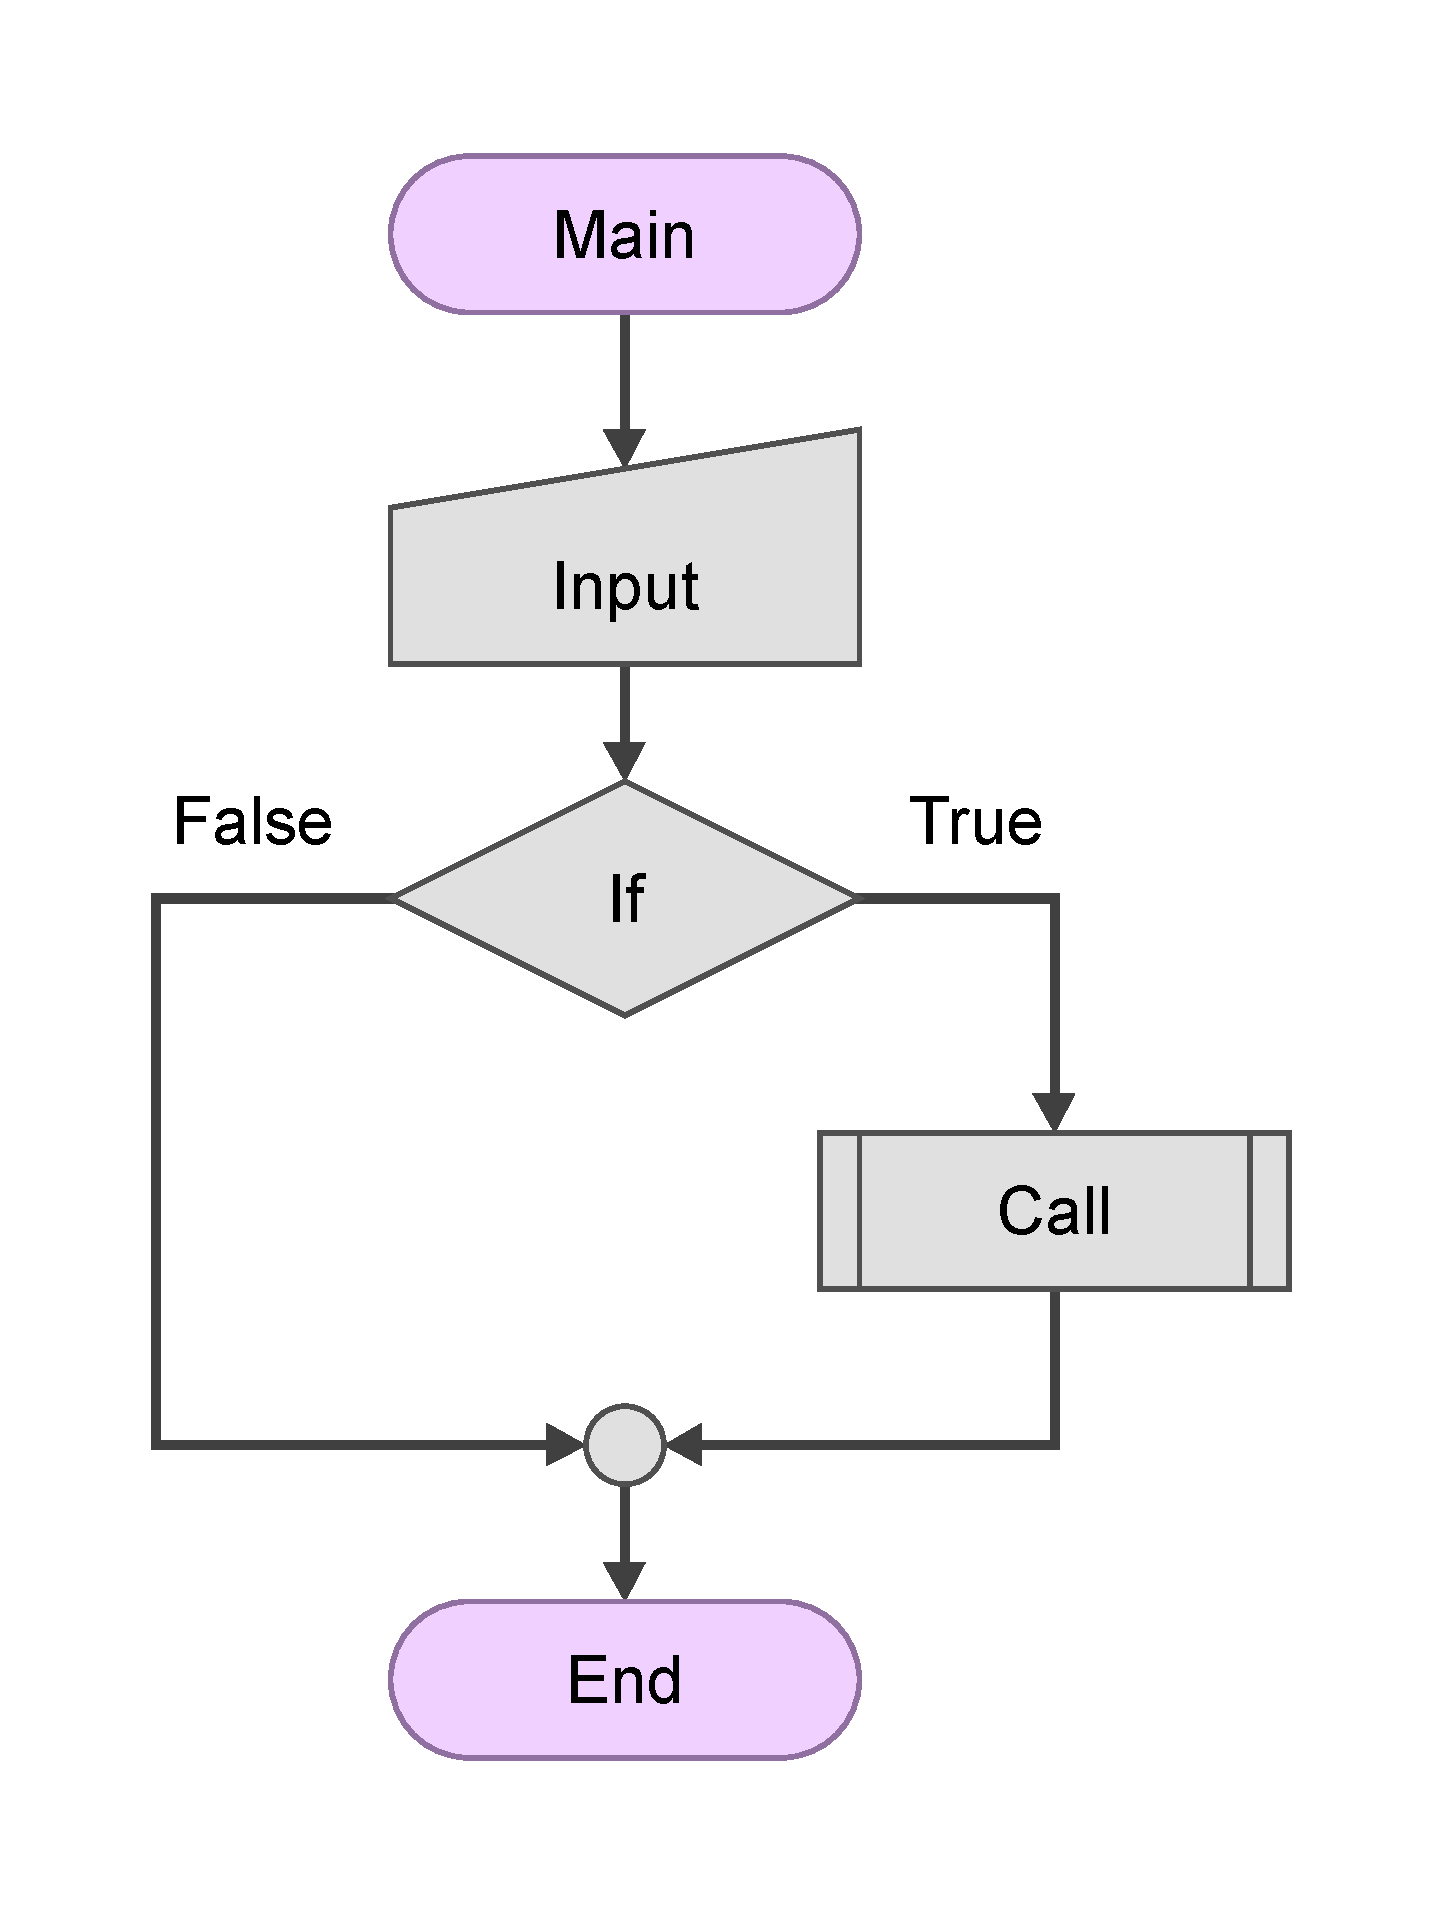
\includegraphics[scale=0.3]{figures/chart.pdf}
    \caption{Example figure in \LaTeX.}
    \label{fig:chart_a}
\end{figure}

\clearpage %  use command \clearpage when you want section or text to appear in the next page.

\section{Example of an algorithm in \LaTeX}
Algorithm~\ref{algo:algo_example} is a good example of an algorithm in \LaTeX.  
\begin{algorithm}
    \caption{Example caption: sum of all even numbers}
    \label{algo:algo_example}
    \begin{algorithmic}[1]
        \Require{$ \mathbf{x}  = x_1, x_2, \ldots, x_N$}
        \Ensure{$EvenSum$ (Sum of even numbers in $ \mathbf{x} $)}
        \Statex
        \Function{EvenSummation}{$\mathbf{x}$}
        \State {$EvenSum$ $\gets$ {$0$}}
        \State {$N$ $\gets$ {$length(\mathbf{x})$}}
        \For{$i \gets 1$ to $N$}                    
        \If{$ x_i\mod 2 == 0$}  \Comment check if a number is even?
        \State {$EvenSum$ $\gets$ {$EvenSum + x_i$}}
        \EndIf
        \EndFor
        \State \Return {$EvenSum$}
        \EndFunction
    \end{algorithmic}
\end{algorithm}
 
\section{Example of code snippet  in \LaTeX}

Code Listing~\ref{list:python_code_ex} is a good example of including a code snippet in a report. While using code snippets, take care of the following:
\begin{itemize}
    \item do not paste your entire code (implementation) or everything you have coded. Add code snippets only. 
    \item The algorithm shown in Algorithm~\ref{algo:algo_example} is usually preferred over code snippets in a technical/scientific report. 
    \item Make sure the entire code snippet or algorithm stays on a single page and does not overflow to another page(s).  
\end{itemize}

Here are three examples of code snippets for three different languages (Python, Java, and CPP) illustrated in Listings~\ref{list:python_code_ex}, \ref{list:java_code_ex}, and \ref{list:cpp_code_ex} respectively.  

\begin{lstlisting}[language=Python, caption={Code snippet in \LaTeX ~and  this is a Python code example}, label=list:python_code_ex]
import numpy as np

x  = [0, 1, 2, 3, 4, 5] # assign values to an array
evenSum = evenSummation(x) # call a function

def evenSummation(x):
    evenSum = 0
    n = len(x)
    for i in range(n):
        if np.mod(x[i],2) == 0: # check if a number is even?
            evenSum = evenSum + x[i]
    return evenSum
\end{lstlisting}

Here we used  the ``\textbackslash clearpage'' command and forced-out the second listing example onto the next page. 
\clearpage  %
\begin{lstlisting}[language=Java, caption={Code snippet in \LaTeX ~and  this is a Java code example}, label=list:java_code_ex]
public class EvenSum{ 
    public static int evenSummation(int[] x){
        int evenSum = 0;
        int n = x.length;
        for(int i = 0; i < n; i++){
            if(x[i]%2 == 0){ // check if a number is even?
                evenSum = evenSum + x[i];
            }
        }
        return evenSum;     
    }
    public static void main(String[] args){ 
        int[] x  = {0, 1, 2, 3, 4, 5}; // assign values to an array
        int evenSum = evenSummation(x);
        System.out.println(evenSum);
    } 
} 
\end{lstlisting}


\begin{lstlisting}[language=C, caption={Code snippet in \LaTeX ~and  this is a C/C++ code example}, label=list:cpp_code_ex]
int evenSummation(int x[]){
    int evenSum = 0;
    int n = sizeof(x);
    for(int i = 0; i < n; i++){
        if(x[i]%2 == 0){ // check if a number is even?
            evenSum = evenSum + x[i];
    	}
    }
    return evenSum;     
}

int main(){
    int x[]  = {0, 1, 2, 3, 4, 5}; // assign values to an array
    int evenSum = evenSummation(x);
    cout<<evenSum;
    return 0;
}
\end{lstlisting}



\section{Example of in-text citation style}
\subsection{Example of the equations and illustrations placement and reference in the text}
Make sure whenever you refer to the equations, tables, figures, algorithms,  and listings for the first time, they also appear (placed) somewhere on the same page or in the following page(s). Always make sure to refer to the equations, tables and figures used in the report. Do not leave them without an \textbf{in-text citation}. You can refer to equations, tables and figures more them once.

\subsection{Example of the equations and illustrations style}
Write \textbf{Eq.} with an uppercase ``Eq`` for an equation before using an equation number with (\textbackslash eqref\{.\}). Use ``Table'' to refer to a table, ``Figure'' to refer to a figure, ``Algorithm'' to refer to an algorithm and ``Listing'' to refer to listings (code snippets). Note that, we do not use the articles ``a,'' ``an,'' and ``the'' before the words Eq., Figure, Table, and Listing, but you may use an article for referring the words figure, table, etc. in general.

For example, the sentence ``A report structure is shown in \textbf{the} Table~\ref{tab:gen_template}'' should be written as ``A report structure is shown \textbf{in} Table~\ref{tab:gen_template}.'' 
 

\section{Summary}
Write a summary of this chapter.

~\\[5em]
\noindent
{\huge\textbf{Note:}} In the case of \textbf{software engineering} project a Chapter ``\textbf{Testing and Validation}'' should precede the ``Results'' chapter. See Section~\ref{subsec:se_chpters} for report organization of such project. 


    \chapter{Results}
\label{ch:results}
This research aims to revolutionize the early identification and prevention of lung-related conditions. Diagnosis of such disease at an advanced level is necessary due to the rise in the number of patients who suffer from such conditions and it should be treated as soon as possible to avoid the growing complexities of respiratory illness. For this, a comprehensive dataset is chosen which contains the X-ray images labeled with four different classes of respiratory conditions. Initially, after analyzing and processing the dataset, it was found that four different respiratory conditions which are “Bacterial Pneumonia”, “Corona Virus Disease”, “Normal”, “Tuberculosis”, and “Viral Pneumonia” are grouped into training, testing, and validation types and a predictive model is built using deep learning and neural network models. The models used are VGG 19, MobileNet, and ResNet and these are provided with these trained image data to recognize patterns that indicate different lung illnesses by closely studying and interpreting the data, which involves sharing and improving expertise. These innovative models are renowned for their precision in picture classification. For this research, Recurrent neural network models are chosen which are VGG 19, MobileNet, and ResNet. After training the VGG 19 model and running it for 20 epochs, it is found that the accuracy of the model is 0.7793 while the accuracy of the MoibleNet model turns out to be around 0.83 which is better than the VGG 19 model. The ResNet model could not show much accuracy as compared to the other models because of which it is discarded and is not trained for further epochs. Therefore, the preferred model with the best accuracy is the MobileNet. These models are further enhanced by using an optimizer like an Adam Optimizer which fine-tunes these models based on certain parameters for promising results.









    \chapter{Discussion and Analysis}

\section{Discussion}
Respiratory-related infections and diseases are a significant obstacle faced worldwide by various health sectors and the general public, especially in old age or places with dense air pollution which leads to deteriorated health conditions. Analyzing such factors manually which cause lung illness is very complicated, laborious, and error-prone, especially in times of global pandemic outbreaks like COVID-19. To better understand four common respiratory diseases—tuberculosis, coronavirus illness, bacterial pneumonia, and normal conditions—this research explores a deep learning-based predictive modeling approach that uses different machine learning and deep learning algorithms to analyze the patient’s medical records for early identification of any traces of lung infection and also preventive measures. The objective of this research is to build an effective healthcare prediction model using different deep learning networks and models that can accurately identify and predict whether the patient is suffering from any classes of lung disease mentioned in the dataset

\section{Summary}
The project explores various processes including predictive modeling techniques like data reading, data analysis where the input dataset is cleaned and modified from raw data to useful data, data processing where the input data is processed for extracting useful information, data visualization where various factors are presented in the form of graphs which is easy to understand and analyze followed by data augmentation where the quality of the input image is enhanced utilizing various techniques like cropping, resizing, upscaling, zooming, etc. All of these processes can be done by using Python libraries like Pandas, Numpy, TensorFlow, and Matplotlib which are built for such tasks. The final step is to deploy various models and train them by providing them with a set of training and testing data. For this research, models like VGG 19, MobileNet, and ResNet are used which are combined with Adam Optimizer and transfer learning which further increases the model’s performance, efficiency, and reliable predictions for any early signs of lung disease. Training these Recurrent Neural Network models is very complex as there are many challenges like underfitting and overfitting, normalization, etc. At last, these models are evaluated based on various performance metrics like classification report, confusion matrix, accuracy score, and F1 score. This research advances the field of predictive analytics in healthcare by combining cutting-edge machine learning approaches with thorough evaluation measures. In the end, it improves patient outcomes globally by assisting healthcare systems in better managing and preventing outbreaks of lung illness.

    \chapter{Conclusions and Future Work}
\label{ch:con}
\section{Conclusions}
For this research, three different Recurrent neural network models are proposed which were utilized to train on the lung data-related outbreak dataset obtained from an online source Kaggle. These models were trained on various aspects and it was seen that the MobileNet model gave the best prediction accuracy out of the other models which are VGG 19 and ResNet chosen for this research. Building such advanced models will revolutionize the working of healthcare institutions in the future as they can detect these deadly diseases at their early stage and thus prevent them with effective measures. Consequently, the standard of care for the impacted patient may be enhanced. 

\section{Future work}
It is crucial to investigate several approaches to increase the prediction model's accuracy and reliability. First, adding more diverse data from different eras and locations to the databases can provide a more comprehensive understanding of the historical and regional evolution of lung disease epidemics. More accurate predictions could result from improving data augmentation methods to more accurately capture the variety and intricacy of lung pictures. It is imperative to evaluate the model in actual healthcare environments and verify its success in early diagnosis and treatment of lung disorders. Experimenting with deep learning architectures other than VGG19, MobileNet, and ResNet may yield fresh perspectives and improve prediction accuracy. By combining many models, experimenting with ensemble learning techniques may also enhance predictions by using the advantages of each approach.  The field of lung disease prediction has the potential to greatly improve patient treatment and international public health outcomes via continuous innovation and improvement of predictive analytics tools. It may be possible to find new approaches to improving prediction models and increasing their effectiveness in managing complex healthcare data by consistently investigating different optimization algorithms.
    \chapter{Reflection}
\label{ch:reflection}
%%%%%%%%%%%%%%%%%%%%%%%%%%%%%%%
%% Please remove/replace text below
%%%%%%%%%%%%%%%%%%%%%%%%%%%%%%%
Write a short paragraph on the substantial learning experience. This can include your decision-making approach in problem-solving.

\textbf{Some hints:} You obviously learned how to use different programming languages, write reports in \LaTeX and use other technical tools. In this section, we are more interested in what you thought about the experience. Take some time to think and reflect on your individual project as an experience, rather than just a list of technical skills and knowledge. You may describe things you have learned from the research approach and strategy, the process of identifying and solving a problem, the process research inquiry, and the understanding of the impact of the project on your learning experience and future work.

Also think in terms of:
\begin{itemize}
    \item what knowledge and skills you have developed
    \item what challenges you faced, but was not able to overcome
    \item what you could do this project differently if the same or similar problem would come
    \item rationalize the divisions from your initial planed aims and objectives.
\end{itemize}


A good reflective summary could be approximately 300--500 words long, but this is just a recommendation.

~\\[2em]
\noindent
{\huge \textbf{Note:}} The next chapter is ``\textbf{References},'' which will be automatically generated if you are using BibTeX referencing method. This template uses BibTeX referencing.  Also, note that there is difference between ``References'' and ``Bibliography.'' The list of ``References'' strictly only contain the list of articles, paper, and content you have cited (i.e., refereed) in the report. Whereas Bibliography is a list that contains the list of articles, paper, and content you have cited in the report plus the list of articles, paper, and content you have read in order to gain knowledge from. We recommend to use only the list of ``References.'' 

    

    
    % -------------------------------------------------------------------
    % Bibliography/References  -  Harvard Style was used in this report
    % -------------------------------------------------------------------
    \bibliographystyle{agsm} % Harvard Style 
    
    \bibliography{references}  %  Patashnik, O. (1988), BibTEXing. Documentation for general BibTEX users.
    
    % -------------------------------------------------------------------
    % Appendices
    % -------------------------------------------------------------------
    
    \begin{appendices}
        \chapter{An Appendix Chapter (Optional)}
\label{appn:A}
% Optional chapter
Some lengthy tables, codes, raw data, length proofs, etc. which are \textbf{very important but not essential part} of the project report goes into an Appendix. An appendix is something a reader would consult if he/she needs extra information and a more comprehensive understating of the report. Also, note that you should use one appendix for one idea.

An appendix is optional. If you feel you do not need to include an appendix in your report, avoid including it. Sometime including irrelevant and unnecessary materials in the Appendices may unreasonably increase the total number of pages in your report and distract the reader.


        \chapter{An Appendix Chapter (Optional)}
\label{appn:B}

...
    \end{appendices}
    
\end{document}
